\chapteropen{Chapter 14: GES: difficult constraints}{chapter-14}
\markboth{Ch. 14 | GES case}{}


\begin{studycolumns}
\vspace{0pt}
\begin{eli5box}
The Grain Elevator System is a practice world for turning one story into many consistent models. A proposed shipment is a plan; a recorded quantity is what actually arrived. Do not add a proposal to the stored amount before the arrival is measured and accepted.
\end{eli5box}
\textbf{Answer check:} Keep proposed and actual grain quantities distinct. Check exact thresholds and started-block charges. A warning is not automatically input rejection. Do not invent sensor-failure, resolution or below-normal policies.


\subsection*{14.1 Domain facts}
\sectionlabel{h-141-domain-facts}

\begin{referenceentries}
\textit{\textbf{Fact} / \textbf{Value}}\par\smallskip
\noindent \textbf{Grain types}: Wheat, barley, long grain rice, short grain rice, oats, hops\par
\noindent \textbf{Grades}: High and low for each grain type\par
\noindent \textbf{Non-empty silo}: Stores only one grain type and grade\par
\noindent \textbf{Empty silo}: May be assigned any accepted grain type and grade\par
\noindent \textbf{Silos}: 12: 1--6 hold 8 000 bushels each; 7--12 hold 12 000 each\par
\noindent \textbf{Total capacity (derived)}: 6 \ensuremath{\times} 8 000 + 6 \ensuremath{\times} 12 000 = \textbf{120 000 bushels}\par
\noindent \textbf{Truck load}: 150--180 bushels\par
\noindent \textbf{Rail car capacity}: 2 000 bushels\par
\noindent \textbf{Arrival}: Trucks from growers/\allowbreak{}sellers only; plate number, driver and seller recorded\par
\noindent \textbf{Departure}: Rail cars to processing plants/\allowbreak{}buyers only; serial number, conductor and buyer recorded\par
\noindent \textbf{Monitoring}: Humidity and temperature sensors send readings periodically\par
\noindent \textbf{Abnormal alert}: \textbf{Sensors} alert both GES and an external grain dryer; affected silo cannot accept more grain until both readings return to normal\par
\end{referenceentries}
The supplement supplies no numeric normal ranges; \textbf{Tutorial 8} supplies those thresholds.


\subsection*{14.2 Hard modelling checks}
\begin{itemize}
\item \textbf{Proposal versus fact:} allocation is a proposed amount per arrival/silo pair. Stock and shipment logs change only after the manager reports actual deposits, whether accepting or overruling the proposal. Partial acceptance is allowed; no-capacity and zero-quantity logging need an agreed policy.
\item \textbf{Overrule is not a bypass:} capacity, compatible grain type/grade and permitted environmental conditions still constrain the chosen silo. Log quantity, type/grade, time, manager, direction, vehicle and the relevant people/organisations.
\item \textbf{Reports:} distinguish capacity remaining for the currently stored type from uncommitted capacity. A pending delivery is not inventory already stored.
\end{itemize}
\subsection*{14.3 Boundary and use-case traps}
GES means tracking software: Manager and directly interacting sensors are actors; Seller/Buyer/Driver/Conductor are recorded entities. Sensors alert the external dryer directly. Arrival includes allocation; optional overrule extends the arrival behaviour. Actual-deposit reporting is required in both paths. Routine use-case descriptions follow Chapter 3's template.
\subsection*{14.4 Class-model traps}
An arrival can use several silos; each silo receives many arrivals over time. An Allocation class carries the proposed amount for that pair. Keep actual deposits distinct. An Arrival uses a Truck; a Departure uses a RailCar. Do not attach both vehicle types to every shipment or assume all business roles inherit Person.
\needspace{4\baselineskip}
\subsection*{14.5 Silo condition state machine (requirement E)}
\sectionlabel{h-145-silo-condition-state-machine-requirement-e}
Model \textbf{environmental condition separately from empty/\allowbreak{}non-empty/\allowbreak{}full}. An empty silo can be abnormal; unloading does not itself restore normal conditions. Sensors, rather than GES, send the dryer alert.


\needspace{375pt}
\par\smallskip\noindent\begin{minipage}{\linewidth}\centering
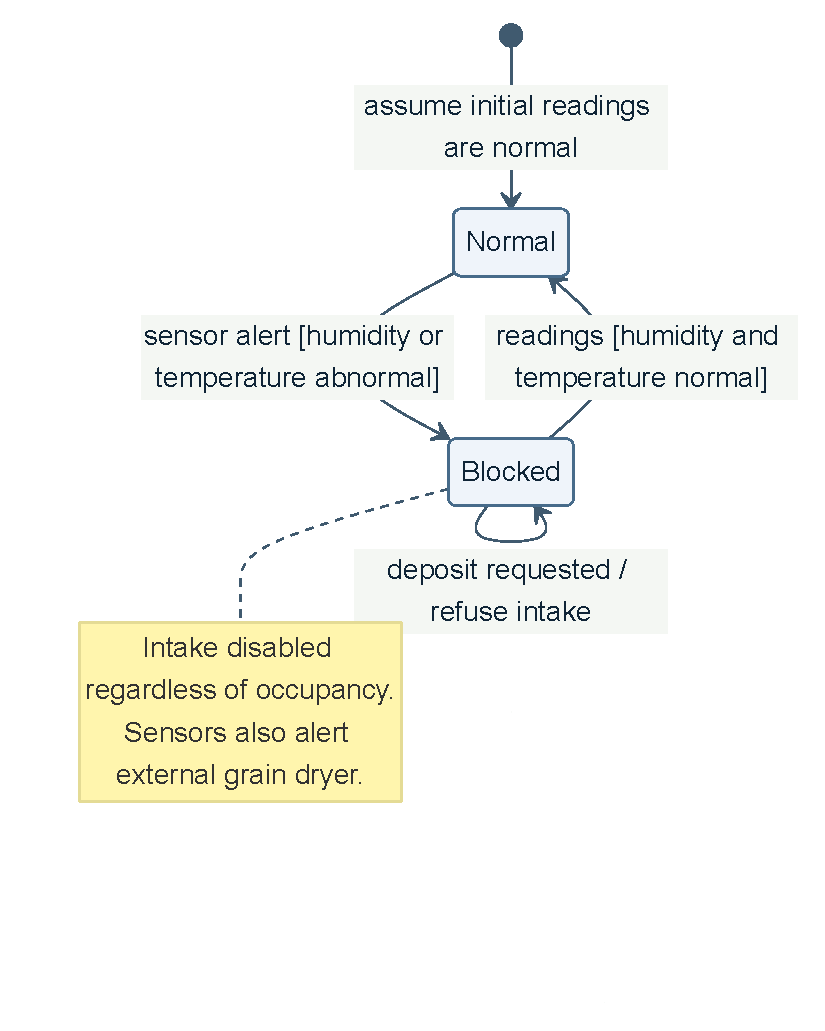
\includegraphics[width=239.91pt]{images/fig-041.pdf}
\captionof{figure}{14.5 Silo condition state machine (requirement E)}\end{minipage}\par\smallskip


The initial normal reading is a stated model assumption. Unknown initial readings and sensor-failure policy remain TBD. ``Intake disabled'' is a constraint; \code{refuse intake} is an event response, not a continuously running \code{do/\allowbreak{}} activity. Returning to Normal removes the sensor block; capacity and type/\allowbreak{}grade constraints still apply.


\subsection*{14.6 Hard arrival invariant}
\textbf{Plan, then record reality:} offer load; compute eligible silo proposal; accept/overrule; unload; report actual amounts and shipment details; update stock/log; acknowledge. Routine class/use-case/sequence drawings are omitted here; the invariants above are the part that cannot be copied blindly from a generic model.
\end{studycolumns}
